\documentclass{article}
\usepackage{graphicx,amsopn,amsthm}


\DeclareMathOperator{\area}{area}
\DeclareMathOperator{\comp}{comp}

 
%\usepackage{amsthm}

\newcommand{\centeripe}[1]{\begin{center}\Ipe{#1}\end{center}}
\newcommand{\comment}[1]{}

\newcommand{\centerpsfig}[1]{\centerline{\psfig{#1}}}

\newcommand{\seclabel}[1]{\label{sec:#1}}
\newcommand{\Secref}[1]{Section~\ref{sec:#1}}
\newcommand{\secref}[1]{\mbox{Section~\ref{sec:#1}}}

\newcommand{\alglabel}[1]{\label{alg:#1}}
\newcommand{\Algref}[1]{Algorithm~\ref{alg:#1}}
\newcommand{\algref}[1]{\mbox{Algorithm~\ref{alg:#1}}}

\newcommand{\applabel}[1]{\label{app:#1}}
\newcommand{\Appref}[1]{Appendix~\ref{app:#1}}
\newcommand{\appref}[1]{\mbox{Appendix~\ref{app:#1}}}

\newcommand{\tablabel}[1]{\label{tab:#1}}
\newcommand{\Tabref}[1]{Table~\ref{tab:#1}}
\newcommand{\tabref}[1]{Table~\ref{tab:#1}}

\newcommand{\figlabel}[1]{\label{fig:#1}}
\newcommand{\Figref}[1]{Figure~\ref{fig:#1}}
\newcommand{\figref}[1]{\mbox{Figure~\ref{fig:#1}}}

\newcommand{\eqlabel}[1]{\label{eq:#1}}
\newcommand{\eqref}[1]{(\ref{eq:#1})}

\newtheorem{thm}{Theorem}{\bfseries}{\itshape}
\newcommand{\thmlabel}[1]{\label{thm:#1}}
\newcommand{\thmref}[1]{Theorem~\ref{thm:#1}}

\newtheorem{lem}{Lemma}{\bfseries}{\itshape}
\newcommand{\lemlabel}[1]{\label{lem:#1}}
\newcommand{\lemref}[1]{Lemma~\ref{lem:#1}}

\newtheorem{cor}{Corollary}{\bfseries}{\itshape}
\newcommand{\corlabel}[1]{\label{cor:#1}}
\newcommand{\corref}[1]{Corollary~\ref{cor:#1}}

\newtheorem{obs}{Observation}{\bfseries}{\itshape}
\newcommand{\obslabel}[1]{\label{obs:#1}}
\newcommand{\obsref}[1]{Observation~\ref{obs:#1}}

\newtheorem{assumption}{Assumption}{\bfseries}{\rm}
\newenvironment{ass}{\begin{assumption}\rm}{\end{assumption}}
\newcommand{\asslabel}[1]{\label{ass:#1}}
\newcommand{\assref}[1]{Assumption~\ref{ass:#1}}

\newcommand{\proclabel}[1]{\label{alg:#1}}
\newcommand{\procref}[1]{Procedure~\ref{alg:#1}}

\newtheorem{rem}{Remark}
\newtheorem{op}{Open Problem}

\newcommand{\etal}{\emph{et al}}

\newcommand{\voronoi}{Vorono\u\i}
\newcommand{\ceil}[1]{\left\lceil #1 \right\rceil}
\newcommand{\floor}[1]{\left\lfloor #1 \right\rfloor}



\title{A Generalized Winternitz Theorem}
\author{Prosenjit Bose \and 
	Paz Carmi \and
	Ferran Hurtado \and
	Pat Morin \and
	Anyone Else?}

\begin{document}
\maketitle
\begin{abstract}
We prove that, for every simple polygon $P$ having $k\ge 1$ reflex
vertices, there exists a point $q\in P$ such that every half-polygon
that contains $q$ contains at least $1/2(k+1)$ times the area of $P$.
We also give a family of examples showing that this result is the best
possible.
\end{abstract}

\section{Introduction}

A classical theorem of Winternitz \cite{X}, that has been rediscovered
many times \cite{a,b,c,d,e}, states that, for any convex polygon $P$,
there exists a point $p\in P$ such that any halfspace that contains
$p$ contains $4/9$ of the area of $P$.  The dissection of a triangle
into 9 similar triangles shown in \figref{dissection} can easily
be used to show that the bound of $4/9$ is tight when $P$ is a triangle.

In this paper, we consider a generalization of Winternitz' Theorem to
the case when $P$ is a simple polygon having $k$ reflex vertices.  A
\emph{chord} of a simple polygon $P$ is a closed line segment whose
interior is contained in in the interior of $P$ and whose endpoints
are on the boundary of $P$.  If $c$ is a chord of $P$ then $P\setminus
c$ has two components $P^+$ and $P^-$.  We call the closure of these
polygons \emph{half-polygons} of $P$.
We define the
\emph{depth} of a point $q\in P$ as 
\[
     \delta_P(q) = \min\{\area(h\cap P) : \mbox{$h$ is a half-polygon
	of $P$ that contains $q$} \} \enspace .
\]
FIXME: Argue that we can assume that $q$ is on the boundary of $h$
because we are taking the minimum.
In this paper, we prove the existence of points with high depth:

\begin{thm}
\thmlabel{lowerbound}
For any simple polygon $P$ with $k \ge 1$ reflex vertices, there 
exists a point $q\in P$ such that $\delta_P(q)\ge \area(P)/2(k+1)$.
\end{thm}
We also show that this bound on $\delta_P(q)$ is the best possible:
\begin{thm}
\thmlabel{upperbound}
For every integer $k\ge 1$ and every $\epsilon > 0$,
there exists a polygon $P$ with $k$ reflex vertices, such that no point
in $P$ has depth greater than  $\area(P)/2(k+1) + \epsilon$.
\end{thm}

The remainder of this paper is dedicated to proving
Theorems~\ref{lowerbound} and \ref{upperbound}.

\section{The Lower Bound}

For simplicity, we will prove a discrete version of
\thmref{lowerbound}.  In the discrete version, we are given a polygon
$P$ and a finite set of points $N \subset P$. The depth of a point $q$
is defined to be the minimal number of points in $N$ contained in the
intersection of $P$ with any half-polygon of $P$ having $q$ on its
boundary.  That is, 
\[
     \delta_{P,N}(q) = \min\{|h\cap N| : \mbox{$h$ is a half-polygon
	of $P$ that contains $q$} \} \enspace .
\]

We first prove the theorem for the case where there is exactly one
reflex vertex ($k=1$).

\begin{clm} 
\label{cl:oneRef}
For any polygon $P$ with one reflex vertex and a finite set $N \subset P$, 
there exists a point $q$ of depth greater or equal to $|N|/4$. 
\end{clm}
%
\begin{proof}

\begin{figure}
   \begin{center}
    %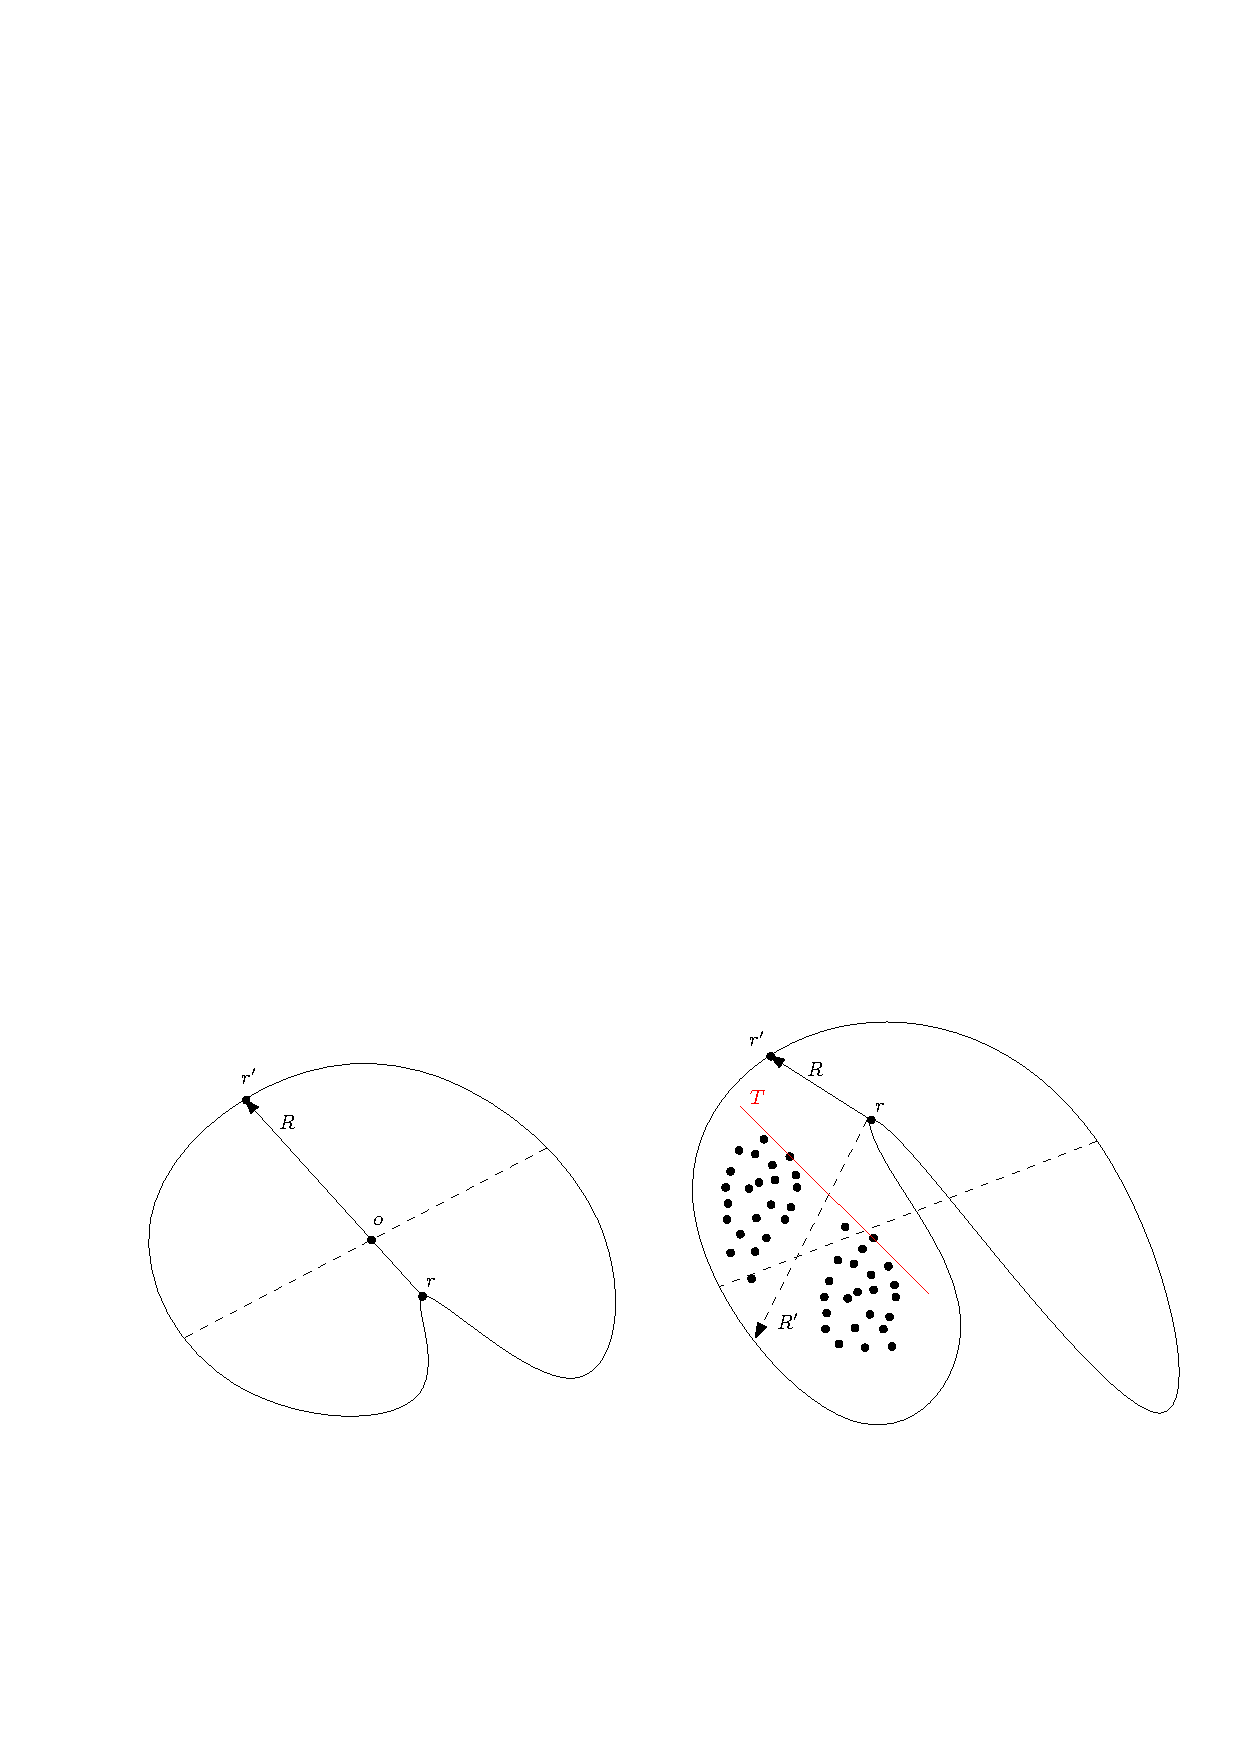
\includegraphics[scale=0.7]{oneReflex.pdf}
   \end{center}
   \caption{lower bound with one reflex vertex}
 \label{fig:tan}
\end{figure}
Let $r$ be $P$'s only reflex vertex.
Draw a ray $R$ emanating from $r$ that divides $P$ 
into two sub-polygons $P_1$ and $P_2$, such that each sub-polygon contains $|N|/2$ points. 
Let $r'$ be the intersection point of $R$ and the boundary of $P$.
By the planar Ham-Sandwich Theorem \cite{ham}, there is a line $\ell$
that splits both $P_1$ and $P_2$ into sub-polygons, each of which contains $|N|/4$ points.
Let $o$ be the intersection point of $\ell$ and $R$.

\begin{enumerate}
\item Point $o$ lies on the segment $\overline{rr'}$. \\
In this case, we set $q=o$ and observe that
each half-plane that contains $o$ contains at least $|N|/4$ points. 
Therefore, the depth of point $o$ is at least $|N|/4$. 

\item Point $o$ does not lay on the segment $\overline{rr'}$. \\
Without loss of generality, assume $P_1$ is a convex polygon (at least one of the two polygons $P_1$ and $P_2$ is convex.)
Draw a ray $R'$ emanating from $r$ that divides $P_1$ 
into two sub-polygons $P'_1$ and $P''_1$, each contains $|N|/4$ points.
For each set of points inside $P'_1$ and $P''_1$, compute the convex hull.
Let $T$ be the tangent of these two convex hulls, such that the half-plane having $T$ on its boundary and not containing $r$ contains all the points in $P_1$ (see Figure~\ref{fig:tan}).
Notice that the intersection point of $T$ and $R'$ has depth of at least $|N|/4$.
 
\end{enumerate} 

\end{proof}

Next, we prove the theorem for a polygon with $k>1$ reflex vertices.
\begin{clm} 
For any simple polygon $P$ with $k>1$ reflex vertices and a set $N \subset P$, 
there exists a point $q$ of depth greater or equal to $\frac{|N|}{2(k+1)}$.
\end{clm}
%
\begin{proof}

\begin{figure}
   \begin{center}
    %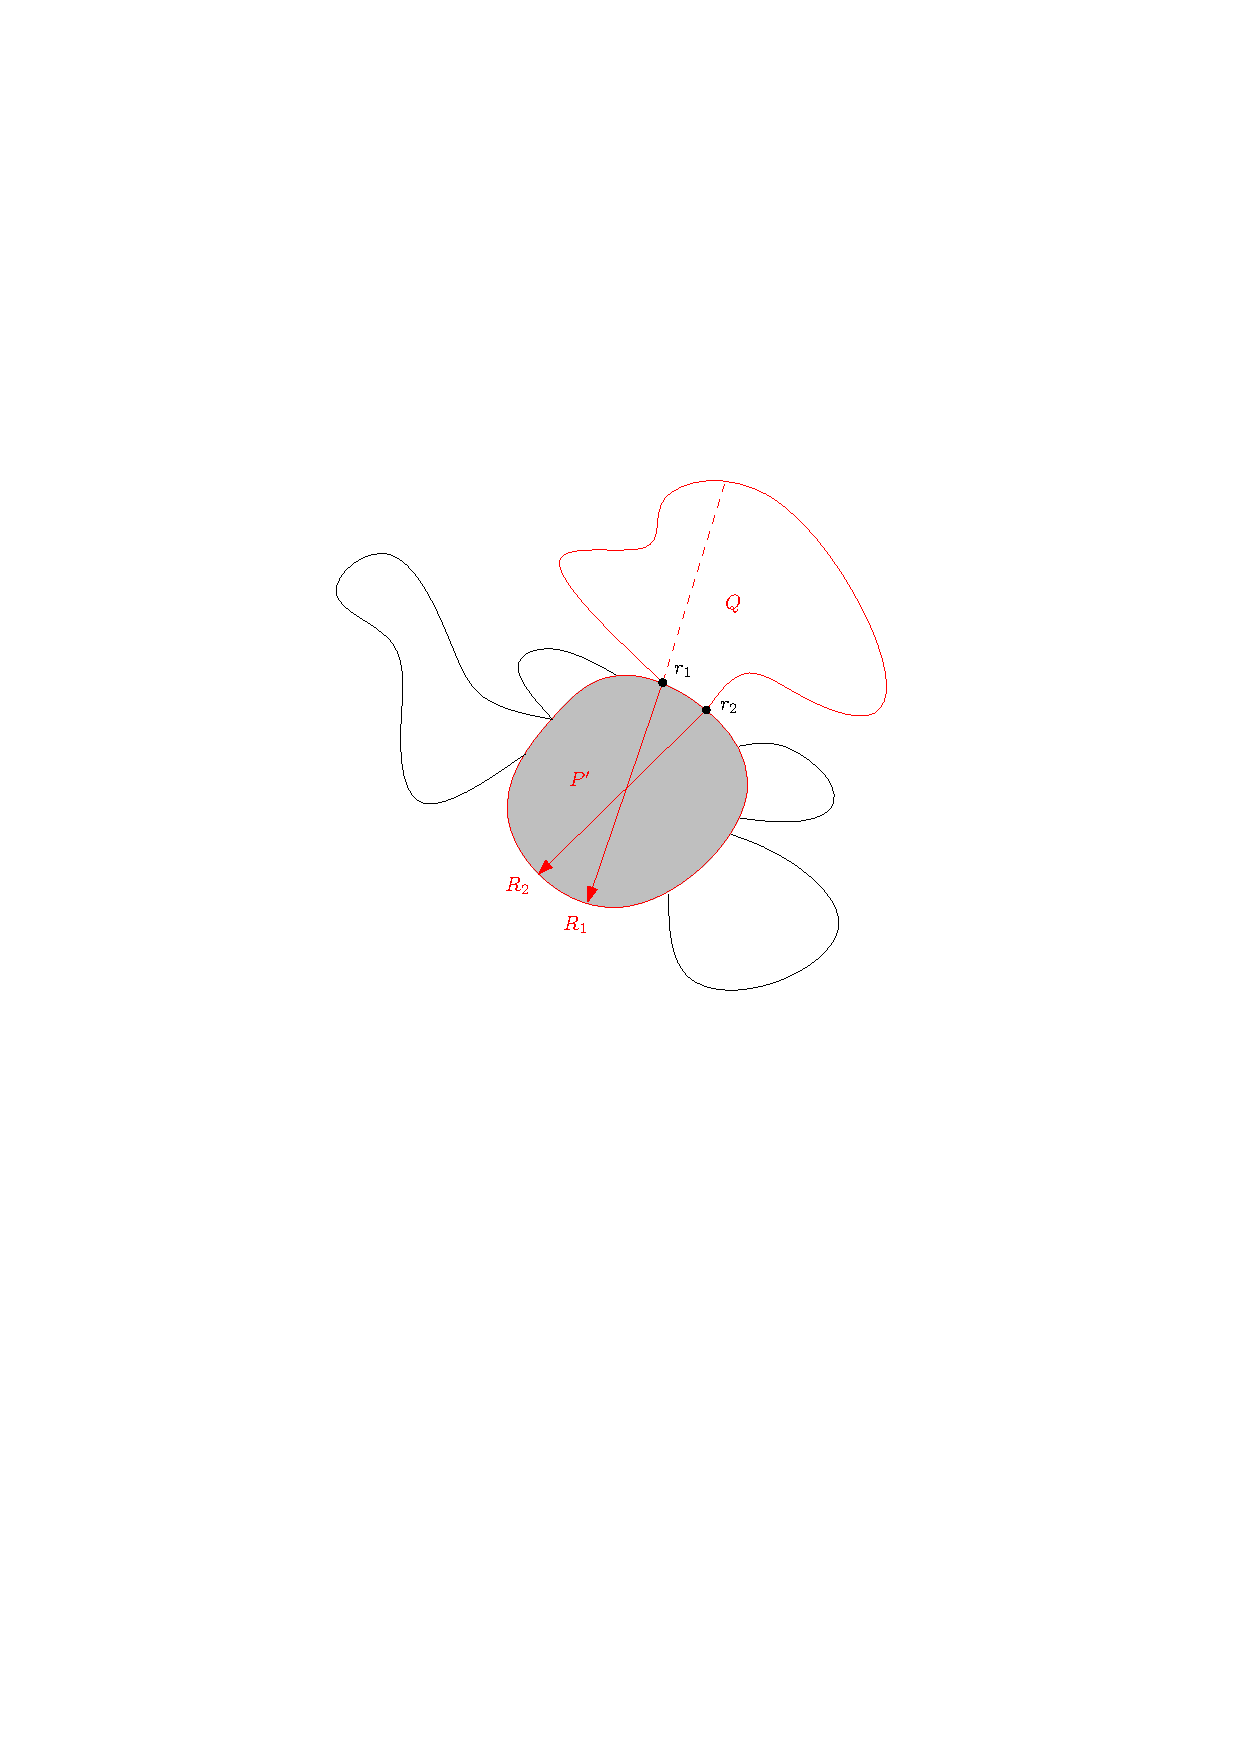
\includegraphics[scale=0.7]{Lowerbound1.pdf}
   \end{center}
   \caption{Lower bound}
 \label{fig:LB1}
\end{figure}

Divide polygon $P$ into at most $k+1$ convex sub-polygons by
iteratively adding a chord on each reflex vertex so that it becomes a
convex vertex in each of the two subpolygons generated.
Let $P'$ be a convex sub-polygon that contains the most points. 
By the pigeonhole principle, $P'$ contains more than
$\frac{|N|}{(k+1)}$ points of $N$. 
Let $Q$ be the component of $P\setminus P'$ containing the largest
number of points of $N$.
Let $(r_1,r_2)$ be line segment that is common to $P'$ and $Q$. 
Draw a chord $R_1$ emanating from $r_1$ that divides $P'$ 
into two sub-polygons $P'_1$ and $P''_1$, each contains $\frac{|N|}{2(k+1)}$ points. 
Similarly, draw a ray $R_2$ emanating from $r_2$ that divides $P'$ 
into two sub-polygons $P'_2$ and $P''_2$, each contains at least $\frac{|N|}{2(k+1)}$ points.
If $Q$ contains less points than $\frac{|N|}{(k+1)}$, then we decrease $P'$, until $Q$ contains  $\frac{|N|}{(k+1)}$ points.

Extend $R_1$ (alternatively $R_2$) in the other direction until it intersects $P$.
This extension divides polygon $Q$ into two sub-polygons $Q_1$ and $Q'_1$ (alternatively $Q_2$ and $Q'_2$).
If the sub-polygon $Q_1$ that does not contain $r_2$ (alternatively $Q_2$ that does not contain $r_1$) 
has more than  $\frac{|N|}{2(k+1)}$ points, then we are done (this is like in Claim~\ref{cl:oneRef} case 2).

Otherwise, we start sweeping from $r_1$ along the edge $(r_1,r_2)$ 
while maintaining that the ray (of the sweep) divides $P'$ into two sub-polygons, 
with the same number of points. 
Notice that we start with sub-polygon $Q_1^*=Q_1$ ($Q_1^*$ represents the expending of $Q_1$ during the sweep)
that has less than $\frac{|N|}{2(k+1)}$ points, and in the end of the sweep 
$Q_1^*$  ($Q_1^*$ contains $r_2$)
%(we denote $Q_1^*$ as $Q_1$ during the sweep) 
contains at least $\frac{|N|}{2(k+1)}$ points. 
%Recall that the sub-polygon of $Q_2$ obtained by the 
%extension of ray $R_2$ in the other direction, that does not contain $r_1$, 
%has less than $\frac{|N|}{2(k+1)}$ points.
Therefore, there is a (balanced) point along the edge $(r_1,r_2)$ in the sweep,
where $Q_1^*$ change the number of points 
it contains from less than $\frac{|N|}{2(k+1)}$ points to at least $\frac{|N|}{2(k+1)}$ points.
The depth of this (balanced) point is at least $\frac{|N|}{2(k+1)}$ 
%
%and there is a point along the edge $(r_1,r_2)$,
%where this sub-polygon (which by now is extended) has at least $\frac{|N|}{2(k+1)}$ points.
%Recall that the sub-polygon of $Q$ obtained by the extension ray $R_2$ in the other direction,
%that does not contain $r_1$, has less than $\frac{|N|}{2(k+1)}$ points.
%Hence, the sub-polygon of $Q$ obtained by the extension ray $R_2$ in the other direction,
%that contains $r_1$, has more or equal to $\frac{|N|}{2(k+1)}$ points.
%Therefore, There must be such a portal (balanced) point along the sweeping, 
%and this point has depth greater or equal to $\frac{|N|}{2(k+1)}$ 
%
(this is similar to Claim~\ref{cl:oneRef} case 1). 

\end{proof}





\section{The Upper Bound}

\begin{proof}[Proof of \thmref{upperbound}]
An example of such a polygon, for the case $k=6$ is shown in
\figref{upperbound}. 

Notice that a point can be located inside or outside a pocket. 
In the former case (inside a pocket), the depth of a point is bounded
by the area of the pocket, which is $\frac{\area(P)}{2(k+1)}$.
In the later case, a point outside a pocket
has a depth smaller than $\frac{\area(P)}{2(k+1)} + \epsilon$. 
FIXME: Do better
\begin{figure}
   \begin{center}
    %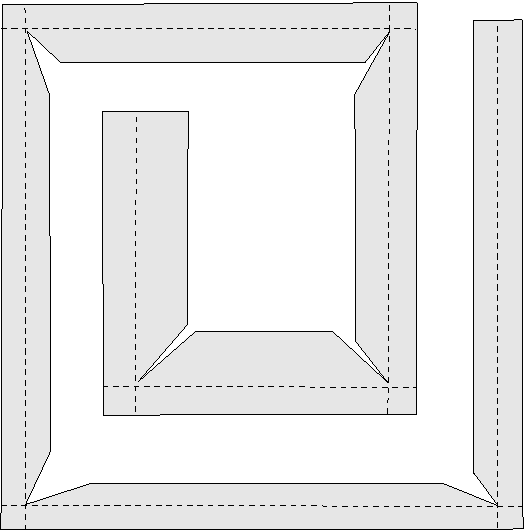
\includegraphics{OneOver2k.pdf}
   \end{center}
   \caption{Upper bound}
 \label{fig:k4}
\end{figure}

\end{proof}

\section{Conclusions}

Open problem: what happens when we consider $\area(h\cap P)$, instead
of $\area(\comp(q,h\cap P))$?



\end{document}

\end{document}
